\documentclass[a4paper,12pt]{report}
\usepackage[utf8]{inputenc}
\usepackage[T1]{fontenc}
\usepackage[ngerman]{babel}
\usepackage[parfill]{parskip}
%\usepackage{eurosans}
\usepackage[top=3cm, left=3cm]{geometry}
\usepackage{setspace}
\usepackage{mdwlist}
\usepackage{graphicx}
\usepackage{eurosym}
\usepackage{tikzsymbols}
\usetikzlibrary{shapes}
\renewcommand*\familydefault{\sfdefault}

\definecolor{esebgcolor}{rgb}{1, 1, 1} % wip-ish color -- #0D5F98
\definecolor{esefgcolor}{rgb}{0,0,0}

\setcounter{secnumdepth}{-1}
\setcounter{tocdepth}{1}
\begin{document}

\title{\huge{\textbf{Vor dem Tutorium lesen und wichtige Punkte markieren!}}\\\ \\\ \\{Leitfaden für ESE-Tutoren 2017}}
\date{}
\author{}
\maketitle

\section*{Anwesenheit in der ESE}
Eure Anwesenheit ist zu folgenden Zeiten ausdrücklich erforderlich:
\begin{itemize*}
	\item Aufgabenbereiche in denen ihr explizit als Helfer eingetragen seid
	\item Frühstück, Tütentragen und Begrüßung am Montag
	\item Bunter Nachmittag am Montag
	\item Einschreibung am Mittwoch
	\item Schnitzeljagd am Donnerstag
	\item ESE-Spiel Am Freitag
	\item Tutorenabschlussgrillen am Freitag 18:00 Uhr
\end{itemize*}
Wichtig für die einzelnen Termine sind auch die vorhering Tutorenbriefings im Ratsaal. Diese sind unbedingt zu besuchen und werden bei nicht erscheinen mit dem Nichterhalt von Goodies geahndet. Man könnte auch sagen, Anwesenheit hat Goodies zur Folge.\\
WICHTIG: Das Briefing am Mittwoch morgen ist die einzige Möglichkeit als nicht-ersti eine ESE Tasse zu erhalten.
Termine für die Briefings sind:
\begin{itemize*}
	\item Montag   		08:30 Uhr
	\item Mittwoch 		08:30 Uhr
	\item Donnerstag	14:00 Uhr
	\item Freitag		12:00 Uhr (Mittag bitte vorher essen)
\end{itemize*}

Die Anwesenheit zu allen anderen Veranstaltungen ist wünschenswert!

\section*{Aufgaben eines ESE-Tutors}

\begin{itemize*}
	\item \textbf{Proud to be a Tutor:} Trage während der Woche zu allen ESE-Veranstaltungen (auch Abends) das ESE-Shirt und dein Namensschild.
	\item \textbf{Präsenz zeigen:} Sei während der ESE so oft wie möglich da, komme zum Frühstück usw. mit den Erstis ins Gespräch.
	\item \textbf{Sei Hilfsbereit:} Siehst du einen einsamen Ersti, hilf ihm, Anschluss zu finden. Ein Ersti fragt dich etwas oder ein Ersti guckt sich verloren um? Setze alles daran zu helfen!
\end{itemize*}

\section*{Ansprechpartner}
Manuel (manuel@ifsr.de): 0176/55140509 \\
FSR/ESE-Orga (ese-orga@ifsr.de): 0351/463-38226 \\

Während der ESE-Woche sollte immer ein Orga-Mitglied im Büro sitzen. Wenn ihr Probleme habt, bitte im Büro anrufen.

\tableofcontents
\chapter{Hinweise für Tutoren}
\section{Himmel statt Scheine}
Scheine gibt es nicht mehr. Zur Motivation haben wir dieses Jahr den Himmel. Der Himmel ist im Raum APB/E008 zu finden und soll als Rückzugsort für euch als Tutoren dienen. Dort könnt ihr euch entspannen und gleichzeitig Feedback an der Tafel hinterlassen. Doch so gemütlich es dort sein mag, solltet ihr doch hin und wieder mal nach draußen gehen und Teil der ESE sein.

\section{Über das Tutorium}
Ziel des Tutoriums ist Vermittlung von Informationen rund um das Studium. Der Inhalt des zweiten Teils dieser Handreichung ist das Minimum, was ihr in den Tutorien vermitteln sollt, ihr könnt die Stichpunkte gerne noch mit eigenen Einfällen ergänzen.\\
Beachtet dabei:
\begin{itemize*}
\item Die Informationen sollten möglichst \textbf{unparteiisch} und \textbf{nicht wertend} vermittelt werden.
Insbesondere sollte man vermeiden, den Erstis schon vorab Angst vor bestimmten Vorlesungen oder Dozenten zu machen oder sie zum Nichtbesuchen der Vorlesungen zu animieren. Das betrifft auch das ESE-Spiel.
\item Eine Tutoriengruppe besteht aus zwei Tutoren und ca. 15-25 Erstis.
\item Solltet ihr zu einem der Themen keine Ahnung haben, dann verweist auf den FSR.
\end{itemize*}

\section{Vor dem Tutorium zu erledigende Dinge}
\begin{itemize*}
\item Überlegt euch wie ihr die Informationen vortragen wollt.
\item Den Raum bitte vorher schon mal suchen, falls ihr nicht sicher wisst, wo er sich befindet.
\item Am ESE-Montag zum Briefing um 08:20 da sein und mit helfen!
\end{itemize*}

\begin{center}
\vspace{1cm}
\begin{tabular}[h]{|l|l|l|l|}
	\hline
	\textbf{Namenspatron}		& \textbf{Raum}	& \textbf{Einschreibezeit}\\ \hline
	Edsger W. Dijkstra			& APB/E005		& 9:00 Uhr\\
	Kurt Gödel					& APB/E006		& 9:10 Uhr\\
	Konrad Zuse					& APB/E007		& 9:20 Uhr\\
	Tim Berners-Lee				& APB/E009		& 9:30 Uhr\\
	John von Neumann			& APB/E010		& 9:40 Uhr\\
	Dennis MacAlistair Ritchie	& WIL/C205		& 9:50 Uhr\\
	Alan Turing 				& WIL/C206		& 10:00 Uhr\\
	Ada Lovelace				& WIL/C203		& 10:10 Uhr\\
	Grace Hopper				& WIL/A221		& 10:20 Uhr\\
	Richard Stallman			& WIL/C107		& 10:30 Uhr\\
	Linus Torvalds				& WIL/B321		& 10:40 Uhr\\
	Noam Chomsky				& WIL/A317		& 10:50 Uhr\\
	Christiane Floyd			& REC/C118		& 11:00 Uhr\\
	Stephen A. Cook				& REC/D16		& 11:10 Uhr\\
	Ken Thompson				& REC/B214		& 11:20 Uhr\\
	Donald Ervin Knuth			& REC/C213		& 11:30 Uhr\\
	\hline
\end{tabular}
\end{center}

\chapter{In den Tutorien zu vermittelnde Informationen}

\section{Einführung}
\begin{itemize*}
\item Wenn ihr Master Studierende in eurer Gruppe habt, schickt sie bitte in den APB E023
\item Fragt für den Spieleabend nach Grillgutestimates. Zur Wahl stehen Steak, Wurst, Grillkäse und Vegane Pommes/Kartoffelecken.
\item Macht eine kleine Vorstellungsrunde, um euch kennenzulernen und die Atmosphäre ein bisschen aufzulockern.
Die Tutoren beginnen. Ihr erzählt, wie ihr heißt, wo ihr ursprünglich herkommt.\\
\textbf{Wichtig!} hierbei geht es nicht um das Studium. Versucht deshalb Fragen zum Studiengang zu vermeiden.\\
Schreibt am besten an die Tafel, was ihr gerne von den Erstis wissen möchtet.
\item Schreibt eure Emailadressen an die Tafel, für Nachfragen.
\item Erzählt etwas zu eurem Namenspatron. Informationen zu diesem findet ihr im Anhang.
\end{itemize*}

\section{ESE-Woche}
\begin{itemize*}
\item ESE-Website: http://ese.ifsr.de (mit aktuellem Ablaufplan der ESE-Woche (da er sich auch in der Woche noch verändern kann), Weblinks, etc.)
\item Den Zeitplan gibt es auch im iCal Format (ICS Datei) auf ese.ifsr.de zum Download.
Kann man sich direkt in den Kalender importieren.
\item Der Ablaufplan der ESE wird am FSR-Büro hinter der Wendeltreppe hängen und auf der ESE-Webseite stehen.
\item Die wichtigen Dinge der ESE-Tüte durchgehen: NoPanic, etc.
\item Geht die ESE-Woche durch und sagt kurz etwas zu den wichtigsten Programmpunkten (siehe Zeitplan und folgende Anmerkungen zu den einzelnen Tagen)
\item Bitte betont nochmal, dass die ESE sehr gut geeignet ist, um Kommilitonen kennenzulernen.
\end{itemize*}
Ort der Begrüßung ist der Hörsaal POT/81 (Pothoff-Bau) und der der Vorträge ist die ganze Woche über die APB/E023.

\textbf{Montag}
\begin{itemize*}
\item 09:00 - 09:45 Frühstück
\item 10:00 - 11:00 Begrüßung im POT/0081
\item 11:00 - 12:00 Tutorien (siehe Tabelle auf S.5)
\item ab 12:00 Mittagspause
  \small{\textit{
  \begin{itemize*}
    \item Geht zusammen mit euren Erstis in die Mensa!
    \item Mensakarten gibt es immer beim Frühstück oder nachher im FSR-Büro
    \item E-Meal aufladen erklären! Automaten, Infopoint, an der Kasse (Zeitersparnis)
    \item Am Nachmittag Sprechstunde im FSR-Büro
  \end{itemize*}
  }}
\item 13:30 - 17:30 Bunter Nachmimttag
  \small{\textit{
  \begin{itemize*}
  	\item Die Führung durch das Lehmann Rechenzentrum ist auf 20 Personen begrenzt.
  	\item Die Führung durch das 5G Lab (5th generation mobile communication systems) ist auch auf 20 Personen begrenzt.
  	\item Die Anmeldung dafür ist am FSR Stand. Die Tatsächlichen Teilnehmer werden ausgelost.
  \end{itemize*}
  }}
\item ab 17:30 Kennenlernspieleabend
\end{itemize*}
\textbf{Dienstag}
\begin{itemize*}
\item Wanderung
  \small{\textit{
  \begin{itemize*}
	\item Treff um 8:15 Uhr Gleis 18 Hauptbahnhof Dresden
	\item Bitte Interesse erfragen
   \end{itemize*}
  }}
\item ab 20:00 Clubwanderung
  \small{\textit{
  \begin{itemize*}
	\item Startet beim Studentenclub CountDown (Güntzstraße 22)
  \end{itemize*}
  }}
\end{itemize*}

\textbf{Mittwoch}
\begin{itemize*}
\item 09:00 - 12:00 Frühstück mit Entertainment, parallel Einschreibung
\item 12:00 - 13:00 Mittagspause
\item ab 13:00 Erstes Seminargruppentreffen
  \small{\textit{
  \begin{itemize*}
    \item jeweils 13:00 und 15:00 je nach Stundenplan/Seminargruppe
    \item zeitgleich dazu finden Vorträge statt.
  \end{itemize*}
  }}
\item ab 20:15 ESE Kino im KiK. Freier Eintritt.
\end{itemize*}


\textbf{Donnerstag}
\begin{itemize*}
\item 09:00 - 09:45 Frühstück
\item 10:00 - 12:00 Vortrag der Lehrpersonen

\item 12:00 - 13:00 Mittagspause
\item 15:00 - 18:00 Campus-Schnitzeljagd
\item 19:00 Impro Theater. Einschreibung über das ifsr Kurssystem (ifsr.de/kurse)
\end{itemize*}

\textbf{Freitag}
\begin{itemize*}
\item 09:00 - 10:00 Frühstück
\item 10:00 - 12:00 Vorträge: Studienangelegenheiten, TUDIAS, Studentische Mitbestimmung, Auslandsstudium.
\item 12:00 - 13:00 Mittagspause
\item 13:00 - 16:00 ESE-Spiel
\end{itemize*}

\textbf{Samstag}
\begin{itemize*}
\item 13:00 - 15:00 Stadtführung
\begin{itemize*}
  \item \small{\textit{bitte erfragt grob das Interesse}}
\end{itemize*}
\end{itemize*}


\subsection{Einschreibung}
\begin{itemize*}
	\item Jede Gruppe hat zugewiesenen Zeitpunkt. Wichtig: Uhrzeit für euer Gruppe ansagen (Siehe Tabelle auf S. 4)!
	\item Empfehlung für Erstis: früh da sein, Einschreibung kann auch schneller gehen. Außerdem gibt ewiges Frühstück mit Entertainment!
	\item Zettel mit Namenspatron unbedingt bis dahin behalten, muss zur Einschreibung vorgezeigt werden (ohne Zettel muss man bis zum Ende der Einschreibung warten)
	\item Mitzubringen sind:
		\begin{itemize*}
		\item Zettel mit Namenspatron
		\item Studentenausweis
		\item ZIH-Login bzw. den ZIH-Coupon (siehe Seite 11)
		\item Wunschstundenplan (vorher raussuchen, sonst kein Einlass!)
		\item zu beachten ist, dass die Einschreiben nur von der Informatik-Fakultät getan werden kann, sie wird erst am Tag danach für außerhalb freigeschalten.
	\end{itemize*}
	\item während der Einschreibung Eintragen in die zwei folgenden Mailinglisten/Mailverteiler möglich (die erste ist ratsam, bei der, auf der Job-Angebote erscheinen, sollte jeder selber wissen ob er das braucht):
		\begin{itemize*}
		\item \textbf{FSR-info} -- FSR Informationen für Studenten.
		\item \textbf{extern} -- Jobangebote werden über diese Mailingliste verbreitet
		\item und diverse andere, siehe \\ https://www.ifsr.de/fsr:news:quicklinks\_fuer\_die\_einschreibung
	\end{itemize*}
\end{itemize*}

\subsection{Seminargruppentreffen}
\begin{itemize*}
	\item Der gewählte Stundenplan bestimmt die Seminargruppe! 
	\item Allgemeiner Sinn der Seminargruppen: Unterstützung der Erstis, Gruppenbildung, Mentor als Ansprechpartner bei Problemen und Vermittlung aller relevanten Informationen zum Studiengang
	\item \glqq Als Einzelgänger kommt man im Studium nicht weit\grqq
	\item Bitte betonen: An allen Treffen teilnehmen!
	\item Erstes Seminargruppentreffen: nach der Einschreibung am Mittwoch um 13 Uhr bzw. 15 Uhr (je nach Seminargruppe - genauer Termin wird bei der Einschreibung dann mitgegeben).
\end{itemize*}
\newpage
\section{Studium}

\subsection{Aufbau und Ablauf}
\begin{itemize*}
	\item Studienjahresablaufplan als Übersicht für die Semester.
	\item Alle wichtigen Infos: Prüfungs- und Studienordnung sowie Studienablaufplan und Modulbeschreibungen findet ihr auf der ESE-Webseite unter Infos - außerdem gibt es ein gedrucktes Exemplar im ersten Seminargruppentreffen
	\item studiengangsspezifische Informationen im ersten Seminargruppentreffen
	\item Studium besteht aus Modulen, Module können Vorlesungen, Übungen, Praktika und Seminare beinhalten:\\
	
	\begin{center}
	Am besten konkret an AuD und Mathe 1 zeigen\\
	Die Zeichnung an die Tafel malen oder was eigenes ausdenken.
  \vspace{0.3cm}
	\end{center}
	\begin{tikzpicture}
    \draw (0,0) rectangle (4,-5);
    \draw (0,0) [fill=black] rectangle (4, -.5);
    \node at (2,0) [below] {\textcolor{white}{Die meisten Module:}};
    \draw (0,-.5) [fill=gray!40] rectangle (4,-1);
    \node at (2,-.5) [below] {bspw. AuD};
    \draw (0,-.5) -- (4,-.5);
    \node (v1) [draw] at (2,-1.6) {Vorlesung};
    \node (u1) [draw] at (2,-2.7) {Übung};
    \draw (0,-3.5) -- (4,-3.5);
    \node (p1) [draw] at (2,-4.3) {Prüfung};
    
    \draw (5,0) rectangle (12, -5);
    \draw (5,0) [fill=black] rectangle (12, -.5);
    \node at (8.5,0) [below] {\textcolor{white}{Spezialfall Mathe im 1. Semester:}};
    \draw (5,-.5) -- (12,-.5);
    \node (pvl) [rectangle,draw,font=\scriptsize] at (8.5,-3.3) [above]{Hausaufgaben};
    \draw (8.5,-.5) -- (pvl);
    \draw (5,-.5) [fill=gray!40] rectangle (8.5,-1);
    \node at (6.75,-.5) [below] {LAG};
    \draw (8.5,-.5) [fill=gray!40] rectangle (12,-1);
    \node at (10.25,-.5) [below] {DIS};
    \draw (5,-1) -- (12, -1);
    \node (v2) [draw] at (6.6,-1.6) {Vorlesung};
    \node (u2) [draw] at (6.1,-2.7) {Übung};
    \node (v3) [draw] at (10.1,-1.6) {Vorlesung};
    \node (u3) [draw] at (10.9,-2.7) {Übung};
    \draw (5,-3.3) -- (12,-3.3);
    \node (p2) [draw] at (7.35,-4) {\glqq{}Nikolausprüfung\grqq{}};
    \node (p3) [draw] at (10.7,-4.4) {Prüfung};
    %\draw[->,thick] (pvl) -- (p3);
  \end{tikzpicture}
  \vspace{0.3cm}\\
  \textit{Die Situation der Mathe-Hausaufgaben ist noch nicht endgültig geklärt - wird bekannt gegeben. Als Prüfungsleistung wird es sie auf jeden Fall nicht geben.}\\

	\item Viele Module: Nur eine Lehrveranstaltung (Vorlesung + Übung)
	\item Jedes Modul hat eine ausgeschriebene Anzahl an Leistungspunkten (LP).\\
	1LP = 30h \glqq Arbeitsbelastung\grqq\ (über das Semester verteilt) bestehend aus:
	\begin{itemize*}
		\item Präsenzzeit (Semesterwochenstunden, SWS)
		\item Vor- und Nachbereitung der Lehrveranstaltung
		\item Vorbereitung auf die Prüfung und Prüfung
	\end{itemize*}
	Leistungspunkte werden einem erst nach bestandener Modulprüfung angerechnet!
\end{itemize*}

\subsection{Vorlesung, Übung, Praktika}
\begin{itemize*}
	\item \textbf{Vorlesung}: meist von einem Professor im Hörsaalzentrum (HSZ) gehalten
	\item \textbf{Übung}: konkrete Aufgaben zur Vorlesung lösen. (So wie in der Schule)
	\item Aufgaben in Übungen entsprechen meist Aufgaben, wie sie in den Prüfungen zu erwarten sind
	\item Angedacht ist: Übungsaufgaben (meist ein A4-Zettel) vor der tatsächlichen Übung vorbereiten $\rightarrow$ in Übung werden dann Ergebnisse besprochen und Fragen geklärt
	\item \textbf{Praktika} = meist uniinterne, praktische Lernveranstaltungen\\
		entweder während der Vorlesungszeit oder als Block in der vorlesungsfreien Zeit
	\item Zur Teilnahme an Vorlesungen, Übungen und Praktika muss man sich einschreiben, im ersten Semester passiert dies über die Stundenpläne, ab dem zweiten Semester schreibt man sich in jede Veranstaltung einzeln ein.
\end{itemize*}
		
\subsection{Prüfungen}
\begin{itemize*}
	\item im Normalfall in der Kernprüfungszeit (ersten 4-5 Wochen der vorlesungsfreien Zeit)
	\item Jedes Modul hat Modulnote:\\
		kann aus verschiedenen Prüfungsleistungen bestehen, die Modulnote ergibt sich wie in der Modulbeschreibung angegeben.
	\item Die Leistungspunkte für ein Modul erhält man erst nach Abschluss aller Modulprüfungen. (Wichtig für BAföG Empfänger)
	\item Theoretisch können eine oder mehrere bestandene Prüfungsvorleistungen (PVL) für Zulassung zu einer Prüfungsleistung nötig sein\\
		\textbf{Beispiel} Mathe: Übungen abgeben $\rightarrow$ 50\% der Übungspunkte müssen erworben sein, um an der zweiten Prüfung teilzunehmen
	\item Mathe-Modul im ersten Semester: \glqq Nikolausklausur\grqq\ in der Mitte des Semesters (erste Prüfungsleistung, zusätzlich zu der am Ende des Semesters)\\
	\textbf{Hinweis:} Mathe im ersten Semester viel Stoff und nicht einfach $\rightarrow$ nicht schleifen lassen!
	\item Prüfungen können zwei mal wiederholt werden
	\begin{itemize*}
		\item 1. Wiederholung: ein Jahr (zwei Semester) Zeit
		\item 2. Wiederholung: zum nächst möglichen Termin
	\end{itemize*}
	2. Wiederholungsprüfung nicht geschafft $\rightarrow$ Exmatrikulation $\rightarrow$ Studium nicht geschafft $\rightarrow$ irgendwas mit Holz!
	\item wieder abmelden von einer Prüfung: ohne Angabe von Gründen bis 3 Werktage (bei schriftlichen Prüfungen) vor dem Prüfungstermin möglich
	\item nach Ende dieser Frist: Rücktritt - nur bei Krankheit o.ä. zulässig\\ 
		muss Prüfungsamt unverzüglich schriftlich mitgeteilt werden (ärztliches Attest o.ä.)
	\item Prüfungsausschuss (je Studiengang): bearbeitet Anträge für Anerkennung bzw. Anrechnung von Studien- und Prüfungsleistungen, Anträge auf Prüfungsfristverlängerung, Anträge auf Annullierung einer Prüfung, etc.
	\item Regelstudienzeit überziehen: sowohl bei Bachelor als auch bei Diplom bis zu 4 Semester, danach Abschlussprüfung das erste Mal nicht bestanden, noch 1 Jahr Zeit für Wiederholung
	\item Studienzeit kann durch Uraubs- und Gremiensemester verlängert werden:
	\begin{itemize*}
		\item Urlaubssemester: studienfreies Semester, in dem auch Prüfungen geschrieben werden können (valider Grund für Urlaubssemester nötig!)
		\item Gremiensemester: max. 3, Reduzierung der Fachsemesterzahl, kann man durch engagierte Gremienarbeit (Fachschaftsrat, Fakultätsrat, Prüfungsausschuss, etc.) bekommen
	\end{itemize*}
\end{itemize*}

\textbf{Einschreibung in Vorlesungen, Übungen und Prüfungen, Abrufen der Prüfungsergebnisse: }elektronische Einschreibesystem jExam (http://jexam.de)\\\\
Eine Zusammenstellung von fürs Studium wichtigen Dokumenten und Links zu vielen Skripten findet man auch auf der FSR-Seite (ifsr.de $\rightarrow$ Studium).
%Diplomer können aufgrund der ähnlichen Lehrveranstaltungen vorerst im Bereich Bachelor nach Skripten gucken, der Bereich \glqq Altes Diplom\grqq\ ist für das \glqq alte\grqq\ Diplom, nicht das neue.

\subsection{Sprachkurse}
\begin{itemize*}
\item Bis zu 10 SWS kostenlose Sprachkurse beim Sprachenzentrum LSK für jeden Studenten
\item Je nach Kurs gibt es Sprachzertifikate
\item Für den Informatik-Master wird Englisch benötigt
\item Webseite: http://lskonline.tu-dresden.de
\end{itemize*}

\section{SLUB}
\begin{itemize*}
	\item Sächsische Landes- und Universitätsbibliothek
	\item für Studenten kostenlos
	\item Online registrieren $\rightarrow$ Karte abholen.
	\item Bücher leihen, ruhige Räumlichkeiten zum Lernen nutzen
	\item Gruppenräume für gemeinsames Arbeiten vorhanden (ggf. reservieren)
	\item Informatikbücher befinden sich in der Lehrbuchsammlung im Haupthaus und im gegenüberliegenden \glqq DrePunct\grqq
\end{itemize*}

\section{Studentische Selbstverwaltung}

\subsection{Fachschaftsrat}
\begin{itemize*}
	\item Auch Erstis können sich gern zur nächsten Wahl für den FSR aufstellen lassen! Alternativ suchen wir für Ende November wieder viele Wahlhelfer!
	\item Vertretung der Studenten auf Fakultätsebene
	\item besteht derzeit aus 17 Mitgliedern
	\item wird immer im Wintersemester für ein Jahr neu gewählt
	\item Ansprechpartner bei Fragen und Problemen
	\item veranstaltet die ESE, Professorenstammtische, die Spieleabende, die Lehrevaluationen, Cyberspace usw.
	\item Sitzungen: jede Woche montags um 18:30 im Großen Ratssaal APB/1004, sind öffentlich, Gäste (gerade Erstis) sind herzlich willkommen
	\item \textbf{FTP-Server (ftp://ftp.ifsr.de):} Protokolle, Klausuren vergangener Jahre, Komplexprüfungsprotokolle (fürs Hauptstudium / Master)
	\item Büro: APB/E017 (hinter der Treppe, neben dem Cafe ascii)	
\end{itemize*}

\subsection{Studentenrat}
\begin{itemize*}
	\item kurz StuRa, Vertretung der Studenten auf Uniebene
	\item Beratungsangebote u.a. zu BAföG, Sozialem und bei Rechtsfragen/-problemen
\end{itemize*}

\subsection{Weitere Ansprechpartner}
\begin{itemize*}
	\item FSR: fsr@ifsr.de
	\item Studiendekan: Prof. Weber (allgemein), Prof. Friedrich (Lehramtsstudiengänge), Prof. Fetzer (englischsprachige Studiengänge).
	\item Studentische Studienberatung: Sascha Peukert (studienberatung-inf@ifsr.de) und Philipp Heisig (studienberatung-minf@ifsr.de) oder beide unter studienberatung@ifsr.de.
	\item Gleichstellungsbeauftragte: http://www.inf.tu-dresden.de/gleichstellung 
	\item Prüfungsamt (APB/3039 und 3040).
\end{itemize*}

\section{Drucken, Kopieren, Rechentechnik}
\begin{itemize*}
	\item ZIH-Login: gilt sowohl fürs Rechenzentrum als auch für jExam, Email und WLAN\\
			Username: \glqq sNummer\grqq
			Jeder Ersti hat einen Coupon erhalten, mit dem er beim ZIH seinen Nutzeraccount aktiviert, ein Passwort setzt und die sNummer bekommt: https://idm-coupon.tu-dresden.de/
  	\item Das Passwort wird für die Einschreibung benötigt!
	\item Jeder Student hat Exchange-Postfach beim ZIH
	\begin{itemize*}
		\item Adresse: sNummer@msx.tu-dresden.de, namensbasierte Weiterleitung \\(vorname.nachname[Zahl]@mailbox.tu-dresden.de)
		\item Abrufen: Outlook/Exchange, IMAP, Webinterface https://msx.tu-dresden.de
		\item \textbf{Wichtig:} regelmäßig abzurufen oder an andere Adresse weiterleiten lassen\\
		$\rightarrow$ Informationen über Prüfungsanmeldung, Rückmeldung zum kommenden Semester etc.
	\end{itemize*}
	\item zwei WLAN-Netze auf dem Uni-Gelände:
	\begin{itemize*}
		\item VPN/Web: wenn möglich vermeiden!
		\item eduroam: auch an anderen Universitäten (sogar international) verwendet\\
		Einrichten: Anleitung auf der Website der TU Dresden\\
		- Login: sNummer@tu-dresden.de
	\end{itemize*}
	\item Rechenzentrum:
	\begin{itemize*}
		\item Computer-Arbeitsplätze (Dualboot mit Windows und Linux - Ubuntu) und Wlan-Arbeitsplätze
		%\item Spezialräume mit Multimedia-Equipment
		\item Technik-Ausleihe (z.B. für Kameras, Beamer, etc.)
	\end{itemize*}
	\item Drucken und Kopieren: 
	\begin{itemize*}
		\item im FSR-Büro (ab 2ct/Seite)
		\item an unterschiedlichen Standorten in der Uni mit beim Stura zu erwerbender Kopierkarte (3,7-5ct/Seite)
		\item in der SLUB (5-15ct/Seite)
		\item an den diversen Copyshops auf dem Unigelände
	\end{itemize*}
	\item MS Imagine (ehemals DreamSpark, ehemals MSDNAA):
	\begin{itemize*}
		\item kostenlose Microsoft Software für Studenten (Windows, Visual Studio,...)
		\item einfach mit ZIH-Login nutzbar
	\end{itemize*}
\end{itemize*}

\section{Studentisches Leben in Dresden}

\subsection{Unisport}
Das Universitätssportzentrum (USZ) bietet viele Sportarten an
\begin{itemize*}
\item Sportprogramm ab 28.10. auf der Homepage des USZ
\item Einschreibung WS 16/17 am 11.10. Nachmittags, gestaffelt nach Sportarten
\item Preise für Studenten recht günstig (zwischen ca. 25-50 Euro pro Semester)
\item Bei begehrten Sportarten schnell sein. viele Kurse nach wenigen Minuten voll
\end{itemize*}

\subsection{ASCII}
\begin{itemize*}
\item Das Studentencafe in der Informatik Fakultät, gleich neben dem FSR Büro.
\item Wird von einem Verein betrieben, bei dem man Mitglied werden kann.
\end{itemize*}

\subsection{Studentenclubs}
\begin{itemize*}
	\item 15 Stück in Dresden (in der Regel Kneipen)
	\item ehrenamtlich von Studenten geführt
	\item  Auflistung z.B. unter http://www.vdsc.de (Vereinigung Dresdner Studentenclubs)
	\item Club, der zur Fakultät Informatik gehört: \glqq CountDown\grqq\ -- kurz: das CD (Nähe Straßburger Platz)\\
	$\rightarrow$ Ausgangspunkt Clubwanderung am Dienstag
\end{itemize*}

\subsection{Kino}
\begin{itemize*}
	\item Studentenkino \glqq Kino im Kasten\grqq
	\item Infos und Programm unter http://kino-im-kasten.de
	\item dort findet am Donnerstag das ESE-Kino statt!
\end{itemize*}


\section{Wohnen in Dresden}
\begin{itemize*}

	\item neuen Wohnsitz innerhalb von 14 Tagen melden
  	\item Hauptwohnsitz nach Dresden verlegen $\rightarrow$ \EUR{150} \glqq Begrüßungsgeld\grqq\\
  $\rightarrow$ beantragen beim Studentenwerk
  \item Zweitwohnungssteuer in Dresden seit 2006 fällig. Bewohner einer WG oder eines Wohnheims kann Widerspruch einlegen
\end{itemize*}

\section{Mensen}
\begin{itemize*}
	\item Emeal-Karte zum zahlen in allen Mensen und Cafeterien der TU Dresden
	\item erhältlich in den Mensen oder ganz einfach während der ESE beim Frühstück oder im FSR-Büro
	$\rightarrow$ Emeal-Bescheinigung (Imma-Bogen), \EUR{5} Kaution, Studentenausweis, Ausweis mitbringen
	\item Aufladen am Automaten in den großen Mensen, an der Kasse (zum Teil nur mit Bargeld möglich), auf Wunsch per Autoload
\end{itemize*}

\section{Grillen}

Fragt bitte die Erstsemester was sie sich für das Grillen am Mittwoch wünschen. Zur Auswahl stehen Steak, Würstchen und Grillkäse. Notiert euch die Mengen und gebt sie an das ESE-Orga Team weiter.

\section{Rundgang durch die Fakultät}
Macht einen kleinen Rundgang durch die Fakultät und zeigt mindestens: ascii, FSR-Büro, E023 (Vorlesungssaal), Rechenzentrum, Prüfungsamt, Ratssaal (1004) mit Hinweis auf FSR Sitzungen. \\
Bietet euren Erstis doch einen Besuch in der Mensa an!
\bigskip
\bigskip
\begin{center}
\huge{\textbf{Geht Mit euren Erstis Mensen!}}
\end{center}
\chapter{Namenspatrone}
\section*{Alan Turing (1912 - 1954)}
\begin{itemize*}
	\item Engländer
	\item schuf den Großteil der theoretischen Grundlagen der modernen Informatik
	\item wirkte wesentlich bei der Entschlüsselung der Enigma im 2. Weltkrieg mit
	\item schrieb das erste Schach-Computerprogramm
	\item entwickelte ein Testverfahren, ob eine Maschine intelligent ist (Turing-Test)
	\item „Nobelpreis“ der Informatik ist nach ihm benannt (Turing-Preis)
	\item Studium: Turing-Maschine (Theoretische Informatik und Logik)
\end{itemize*}

\section*{Edsger W. Dijkstra (1930 - 2002)}
\begin{itemize*}
	\item Niederländer
	\item Djikstra-Algorithmus zur Berechnung des kürzesten Wegs in einem Graphen
	\item Semaphore zur Synchronisation von Threads
	\item berühmt wegen Abhandlung ``Goto considered harmful''
	\item Einführung der strukturierten Programmierung (verwendet in Programmiersprachen wie
	      Pascal oder C)
	\item Studium: Dijkstra-Algorithmus (Algorithmen und Datenstrukturen), Semaphore
	      (Betriebssysteme und Sicherheit)
\end{itemize*}

\section*{Kurt Gödel (1906 - 1978)}
\begin{itemize*}
	\item Deutscher
	\item Beiträge zur Relativitätstheorie und klassischen Logik
	\item viele Beiträge zur Prädikatenlogik (Vollständigkeit und Entscheidungsproblem)
  	\item Entwicklung der Gödelnummer einer Turing-Maschine
  	\item Studium: Prädikatenlogik, Gödelnummer (Theoretische Informatik und Logik)
\end{itemize*}

\section*{Konrad Zuse (1910 - 1995)}
\begin{itemize*}
	\item Deutscher
	\item gilt als Erfinder des modernen Computers
	\item Konstruktion der Computer Z1 bis Z4
	\item Entwicklung der ersten höheren Programmiersprache „Plankalkül“
	\item theoretische und praktische Arbeit zur Darstellung von Gleitkommazahlen (Exponent,
		  Mantisse)
	\item Studium: Gleitkommazahlen, Vektorrechner (Rechnerarchitektur)
\end{itemize*}

\section*{Donald Ervin Knuth (geb. 1938)}
\begin{itemize*}
	\item Amerikaner
	\item Verfasser von „The Art of Computer Programming“ (Standardwerk über Datenstrukturen \&
		  Algorithmen)
	\item entwickelte das Satzsystem TeX
	\item Erfinder des KMP-Algorithmus (String Matching) und des Buddy-Verfahrens
	      (Speicherverwaltung)
	\item Studium: KMP-Algorithmus (Algorithmen und Datenstrukturen), Buddy-Algorithmus
		  (Betriebssysteme und Sicherheit)
\end{itemize*}

\section*{John von Neumann (1903 - 1957)}
\begin{itemize*}
	\item Österreicher
	\item Beiträge in Quantenmechanik und Spieltheorie
	\item Entwicklung der von-Neumann-Architektur
	\item Studium: von-Neumann-Architektur, Binäre Kodierung (Rechnerarchitektur)
\end{itemize*}

\section*{Tim Berners-Lee (geb. 1955)}
\begin{itemize*}
	\item Engländer
	\item gilt als Begründer des World Wide Web (Web-Developer \Laughey)
	\item erfand HTML
	\item schrieb den ersten Browser
	\item Vorsitzender des W3C (Gremium, welches grundlegende Standards des Netzes
	      spezifiziert)
	\item Studium: WWW (Rechnernetze)
\end{itemize*}

\newpage

\section*{Ada Lovelace (1815 - 1852)}
\begin{itemize*}
	\item Engländerin
	\item gilt als erste Programmiererin der Welt
	\item beschrieb, wie man die Bernoulli-Zahlen mit einer Maschine berechnen kann
	\item Namensgeberin der Programmiersprache Ada
\end{itemize*}

\section*{Grace Hopper (1906 - 1992)}
\begin{itemize*}
	\item Amerikanerin
	\item 1954 ersten Compiler (A-0) entwickelt
	\item fand den ersten (Hardware) Bug (heißt Bug, weil es eine Motte war)
	\item Studium: Entwicklung der Rechentechnik (Rechnerarchitektur)
\end{itemize*}

\section*{Richard Stallman (geb. 1953)}
\begin{itemize*}
	\item Amerikaner
	\item Präsident der Free Software Foundation
	\item entwickelte die GNU Public License (GPL)
	\item entwickelte die ersten Versionen einiger GNU-Tools (gcc, gdb und Emacs)
\end{itemize*}

\section*{Linus Torvalds (geb. 1969)}
\begin{itemize*}
	\item Finne
	\item Initiator des freien Kernels Linux
	\item bis heute einer der führenden Entwickler von Linux
	\item Studium: Linux (Betriebssysteme und Sicherheit)
\end{itemize*}

\section*{Noam Chomsky (geb. 1928)}
\begin{itemize*}
	\item Amerikaner
	\item Beiträge in verschiedenen Bereichen wie Linguistik und Psychologie
	\item Chomsky-Hierarchie teilt formale Sprachen in Klassen (Typ 0 bis Typ 3) ein
	\item wichtige Grundlage der Theoretischen Informatik, speziell des Compilerbaus
	\item Studium: Chomsky-Hierarchie (Formale Systeme)
\end{itemize*}

\newpage

\section*{Christiane Floyd (geb. 1943)}
\begin{itemize*}
	\item Österreicherin
	\item erschuf die erste Entwicklungsumgebung Maestro I
	\item erste Professorin im Bereich Informatik in Deutschland
	\item umfangreiche Forschung im Bereich von Softwarentwicklungsmethoden
\end{itemize*}

\section*{Stephen A. Cook (geb. 1939)}
\begin{itemize*}
	\item Amerikaner
	\item forscht hauptsächlich im Bereich der Theoretischen Informatik
	\item formulierte in seinem berühmtesten Paper den Begriff der NP-Vollständigkeit
	\item lässt die Frage, ob P=NP ist, offen $\rightarrow$ eine der zentralen Fragestellungen
	      der modernen Informatik („Preisgeld“: \$ 1.000.000)
	\item Studium: NP-Vollständigkeit (Theoretische Informatik und Logik)
\end{itemize*}

\section*{Ken Thompson (geb. 1943)}
\begin{itemize*}
	\item Amerikaner
	\item entwickelte Programmiersprache B (Vorgänger von C)
	\item erschuf mit Dennis Ritchie erste Version von UNIX
	\item schrieb frühe Versionen von Tools wie der ersten Shell sh, die bis heute Bestandteil
	      moderner Betriebssysteme sind
	\item Studium: Unix (Betriebssysteme und Sicherheit)
\end{itemize*}

\section*{Marc Andreessen (geb. 1971)}
\begin{itemize*}
	\item Amerikaner
	\item Mitbegründer der Netscape Corp.
	\item schrieb einen der ersten weit verbreiteten Browser Mosaic
	\item entwickelte mit am Netscape Navigator, der die Grundlage vom Mozilla Firefox ist
\end{itemize*}

\section*{Rudolf Bayer (geb. 1939)}
\begin{itemize*}
	\item Deutscher
	\item forscht im Bereich der Datenbanken
	\item entwickelte Datenstruktur B-Bäume (Grundlage der meisten modernen Datenbank- und
		  Dateisysteme)
	\item Studium: B-Bäume (Datenbanken)
\end{itemize*}

\section*{Dennis MacAlistair Ritchie (1941 - 2011)}
\begin{itemize*}
	\item Amerikaner
	\item entwickelte mit Ken Thompson Unix
	\item erschuf die Programmiersprache C
	\item Studium: C (Algorithmen und Datenstrukturen), Unix (Betriebssysteme und Sicherheit)
\end{itemize*}

\section*{Claude Shannon (1916 - 2001)}
\begin{itemize*}
	\item Amerikaner
	\item beschäftigte sich mit mathematischen Grundlagen der Kommunikation
	\item Definition von Begriffen wie Information und Entropie
	\item Studium: Nyquist-Shannon-Abtasttheorem, Shannon-Fano-Verfahren (Informations- und
	      Kodierungstheorie, Rechnernetze, Einführung in die Medieninformatik)
\end{itemize*}

\section*{C.A.R. Hoare (geb. 1934)}
\begin{itemize*}
	\item Brite
	\item beschäftigte sich mit den theoretischen Grundlagen von Programmiersprachen
	\item entwickelte Hoare-Kalkül (Korrektheit von Algorithmen)
	\item erfand Quicksort
	\item Studium: Hoare-Kalkül (Programmierung), Quicksort (Algorithmen und Datenstrukturen)
\end{itemize*}

\section*{Alonzo Church (1903 - 1995)}
\begin{itemize*}
	\item Amerikaner
	\item Mathematiker und Logiker
	\item erfand den Lambda-Kalkül (Grundlage funktionaler Programmiersprachen)
	\item führte den Begriff der intuitiven Berechenbarkeit ein (Church-Turing-These)
	\item Studium: Lambda-Kalkül (Programmierung), Berechenbarkeit (Theoretische Informatik
		  und Logik)
\end{itemize*}

\pagebreak

\begin{tikzpicture}[timebox/.style={draw,text=esefgcolor,fill=esebgcolor,font=\scriptsize\bfseries,align=left}]
    \node at (0,0) {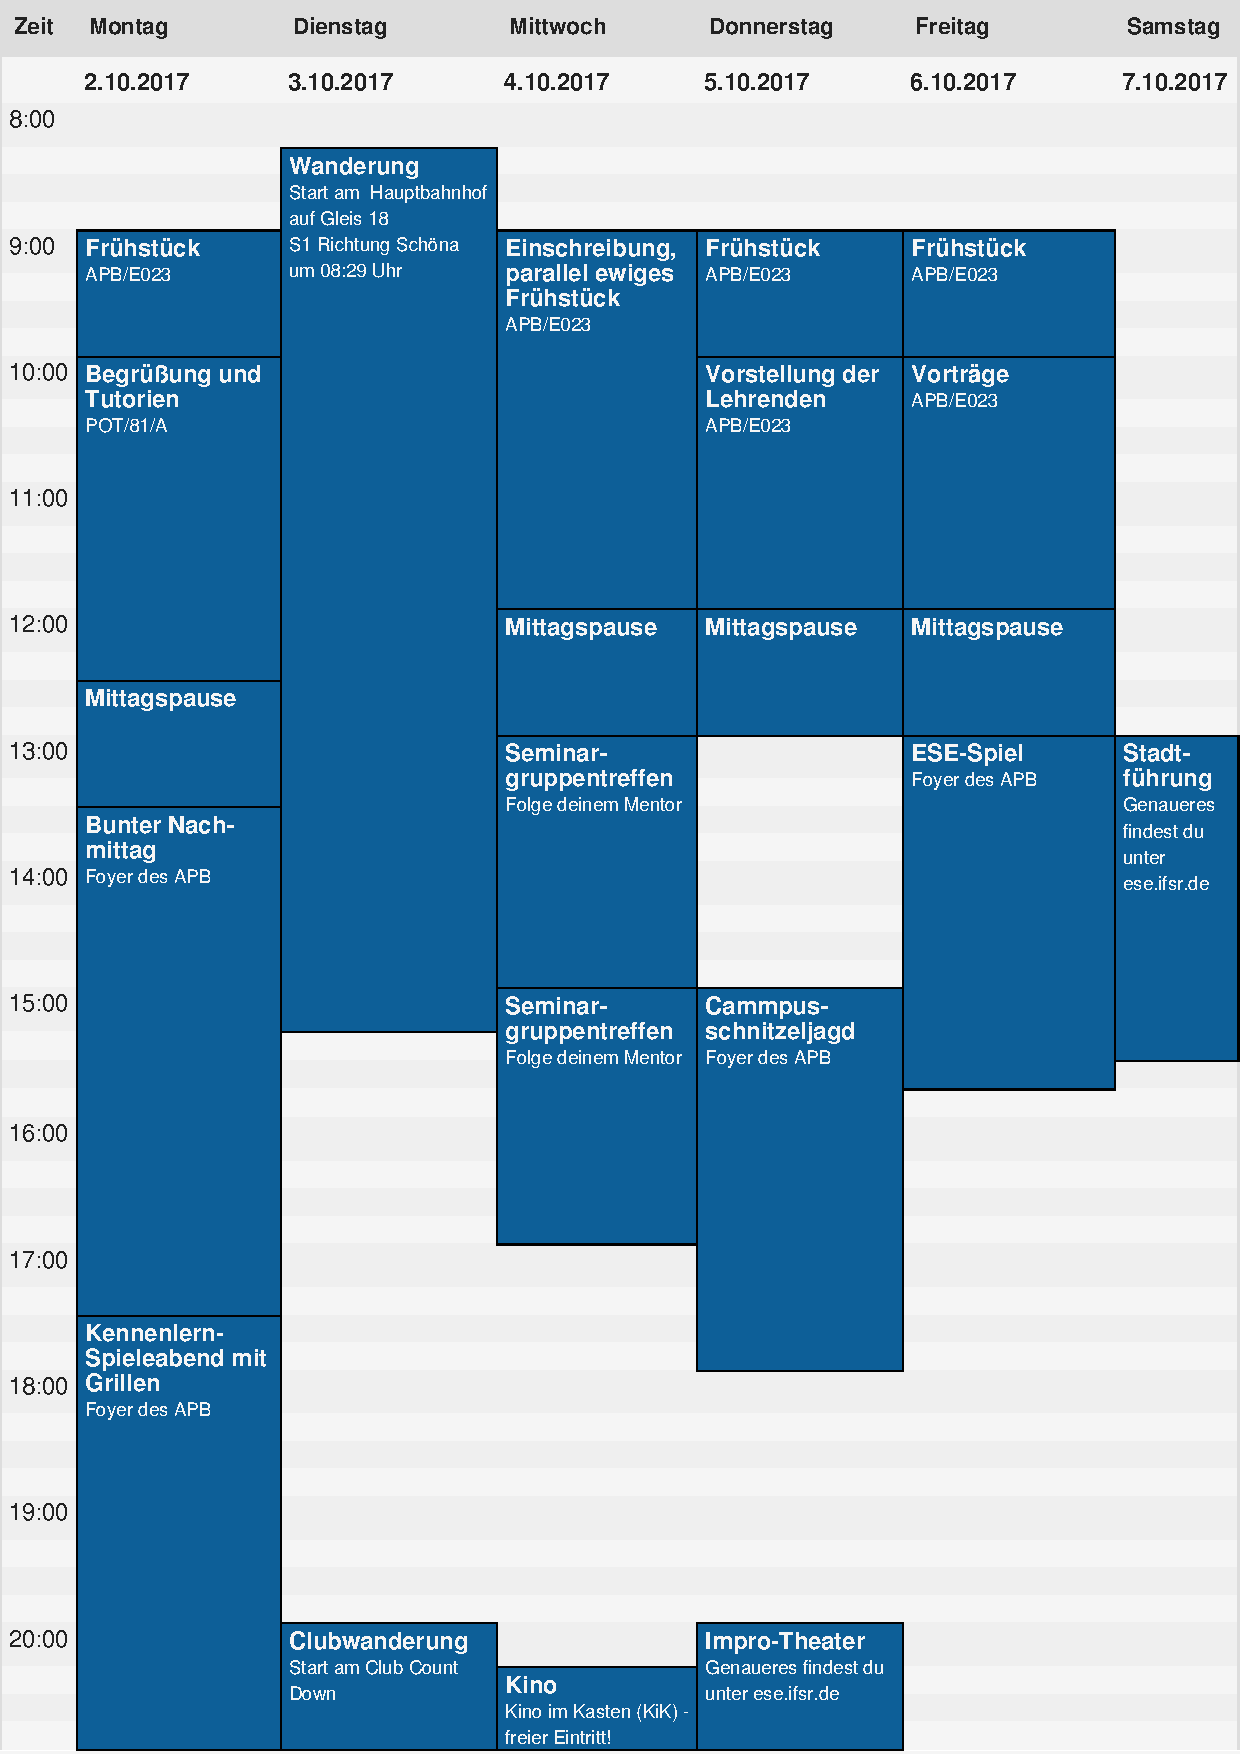
\includegraphics[width=\linewidth]{zeitplan_2017.pdf}};
    \node[timebox,text width=2.165cm,minimum height=0.99cm] at (-5.28,8.235) {8:30\\Tutorenbriefing};
    \node[timebox,text width=2.12cm,minimum height=0.99cm] at (-0.27,8.235) {8:30\\Tutorenbriefing};
    \node[timebox,text width=2.2cm,minimum height=1.5cm] at (2.16,-0.59) {14:00\\Tutorenbriefing\\\ \\};
    \node[timebox,text width=2.25cm,minimum height=1.505cm] at (4.665,2.44) {12:00\\Tutorenbriefing\\\ \\};
    \node[timebox,text width=2.18cm,minimum height=4.535cm] at (4.64,-8.19) {18:00\\ Tutorengrillen\\\ \\\ \\\ \\\ \\\ \\\ \\\ \\\ \\\ \\\ \\};
\end{tikzpicture}

\end{document}
